
      


\subsection{VOTE dataset}

We present the experimental results with the VOTE dataset in~\Cref{fig:vote_results}. Experiments were conducted with both weak and strong confounders, and under small and large sample regimes. We use the outcome $Y$ as a strong confounder given the lack of a feature highly correlated with the outcome in the dataset. These results corroborate previous findings that higher correlated confounders and larger sample sizes lead to greater power of our test. In all scenarios, the performance of both tests closely aligns.

\begin{figure*}[hb]
    \begin{subfigure}[b]{0.24\textwidth}
        \centering
    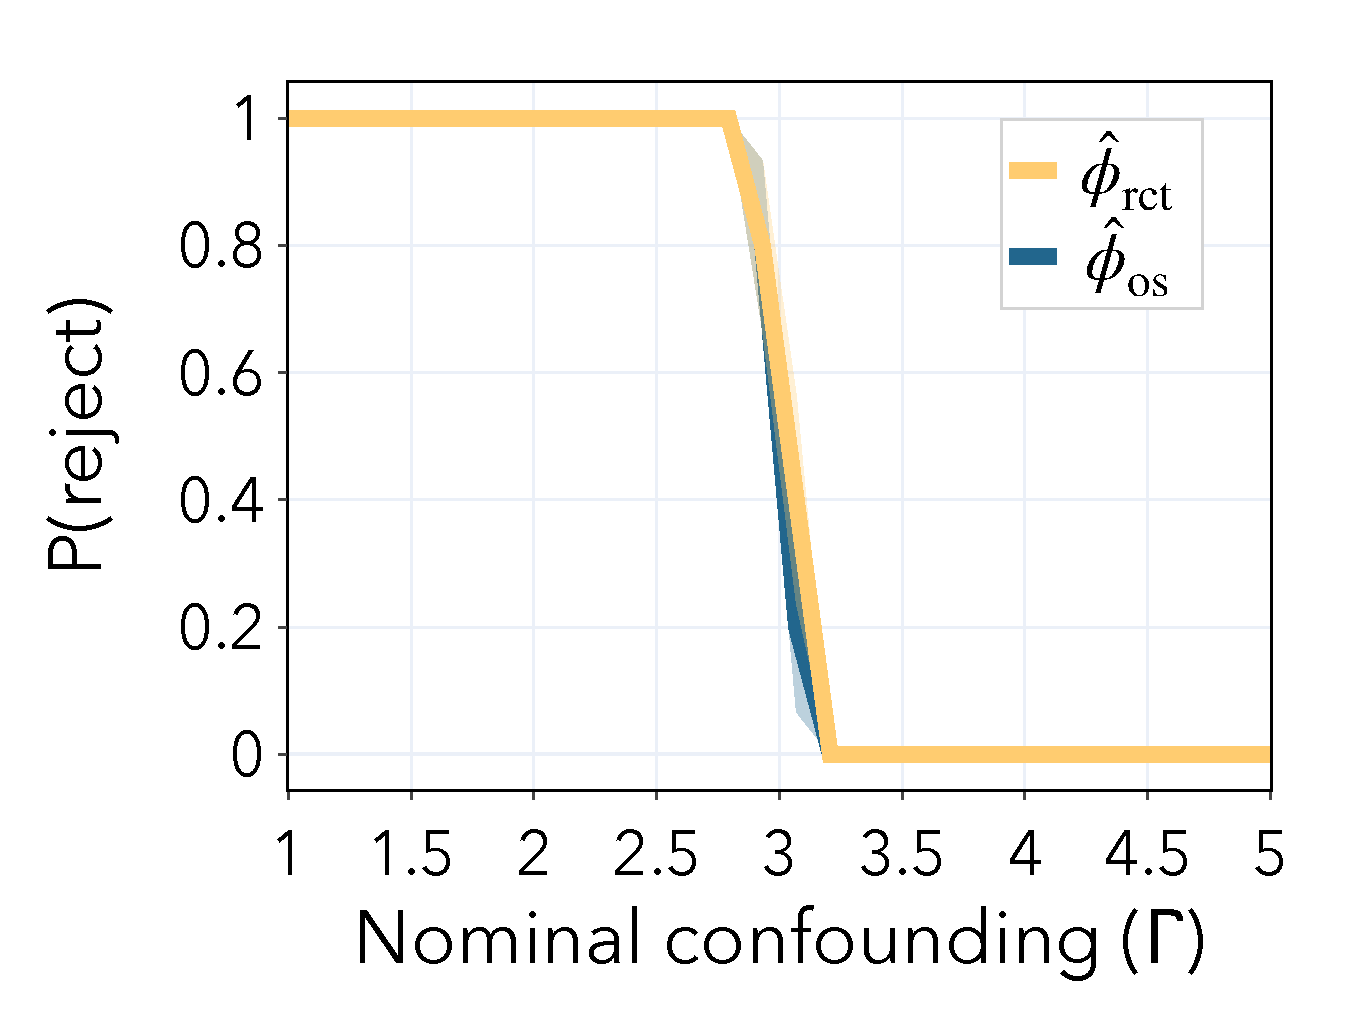
\includegraphics[width=\textwidth]{vote_weak_small.pdf}
        \caption{Small sample ``age"}
        \label{vote:weak_small}
    \end{subfigure}
    \hfill
    \begin{subfigure}[b]{0.24\textwidth}
        \centering
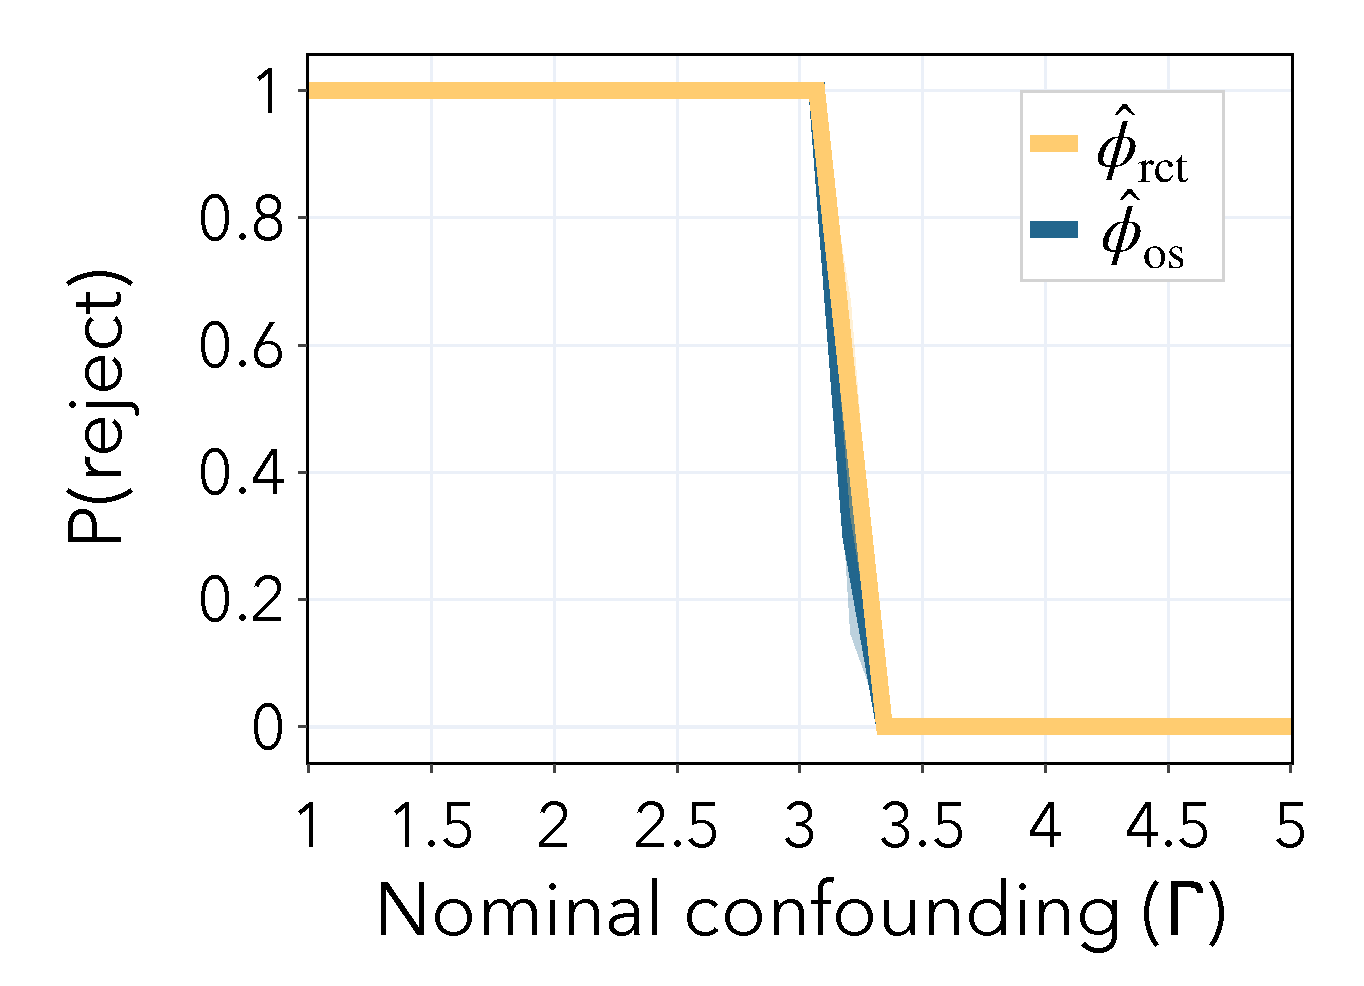
\includegraphics[width=\textwidth]{vote_weak.pdf}
        \caption{Large sample ``age"}
        \label{vote:weak_large}
    \end{subfigure}
    \hfill
    \begin{subfigure}[b]{0.24\textwidth}
        \centering
   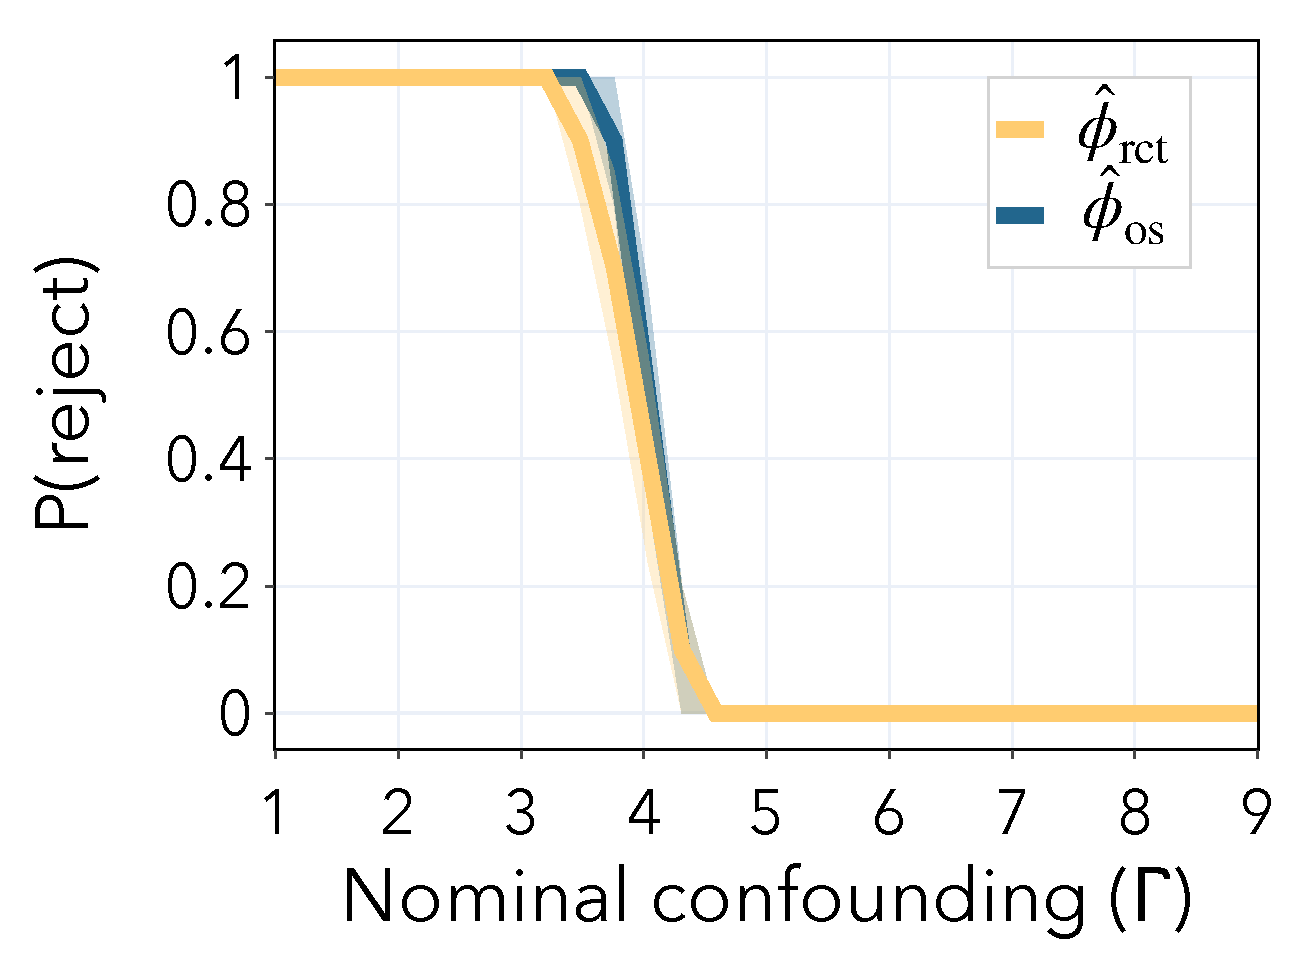
\includegraphics[width=\textwidth]{vote_strong_small.pdf}
        \caption{Small sample $Y$}
        \label{vote:strong_small}
    \end{subfigure}
    \hfill
    \begin{subfigure}[b]{0.245\textwidth}
        \centering
    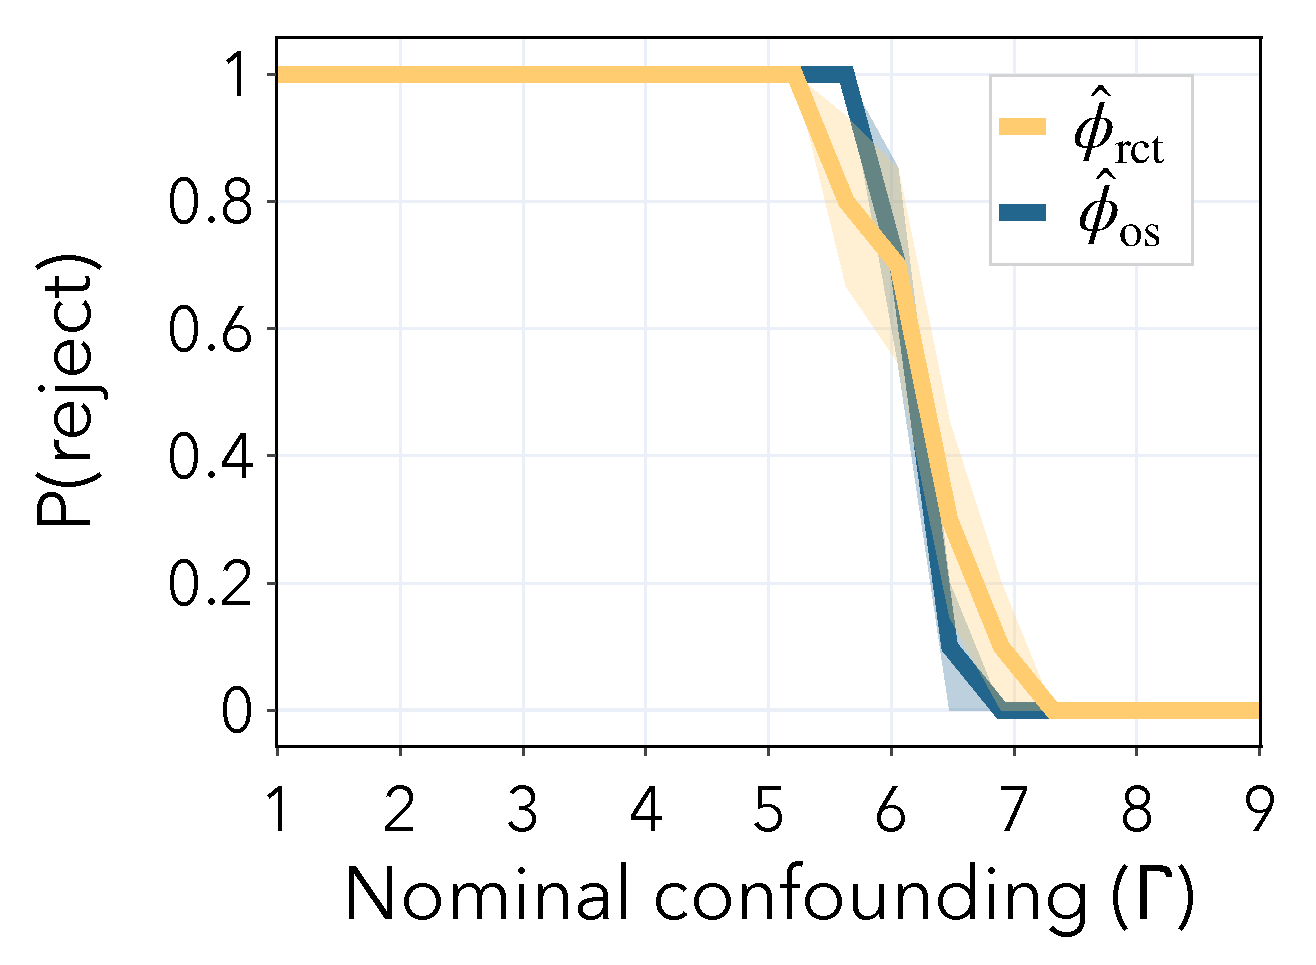
\includegraphics[width=\textwidth]{vote_strong.pdf}
        \caption{Large sample $Y$}
        \label{vote:strong_large}

    \end{subfigure}
    
    \caption{Probability of rejection for different choices of $\confvalue$ for the test for the VOTE dataset. For all the plots, the significance level is $\alpha=0.05$ and $\Gammatrue=9$. (a)-(b) Weak confounder: ``age". (a) small sample size: $\nrct=3.2K,\nobs=11K$ and (b) large sample size: $\nrct=10.6K,\nobs=36.8K$. (c)-(d) Strong confounder: outcome $Y$. (c) small sample size: $\nrct=3.2K,\nobs=11K$ and (d) large sample size: $\nrct=10.6K,\nobs=36.8K$.
 }
    \label{fig:vote_results}
\end{figure*}

\subsection{Tennessee STAR Project}

 We present the experimental results with the STAR Project in~\Cref{fig:star_results}. Experiments were conducted with both weak and strong confounders with the full dataset. We do not run experiments with a small sample size since the STAR dataset already represents a small sample regime. These results corroborate previous findings that higher correlated confounders lead to greater power. 
 
\begin{figure*}[b]
\centering
    \begin{subfigure}[b]{0.3\textwidth}
        \centering
    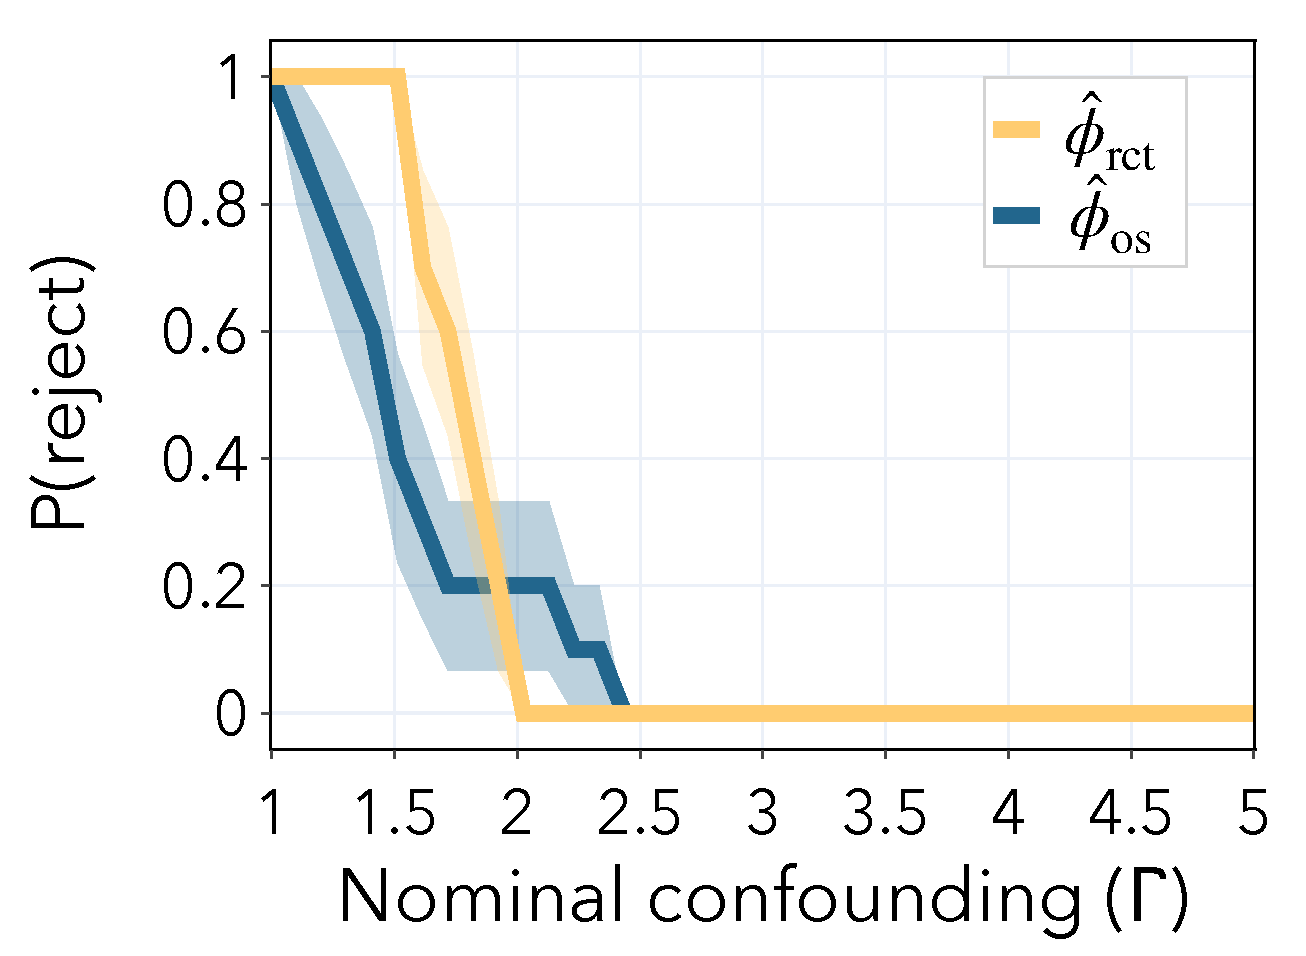
\includegraphics[width=\textwidth]{star_weak.pdf}
        \caption{Weak confounder: ``free lunch"}
        \label{star:weak}
    \end{subfigure}%
    \begin{subfigure}[b]{0.3\textwidth}
        \centering
    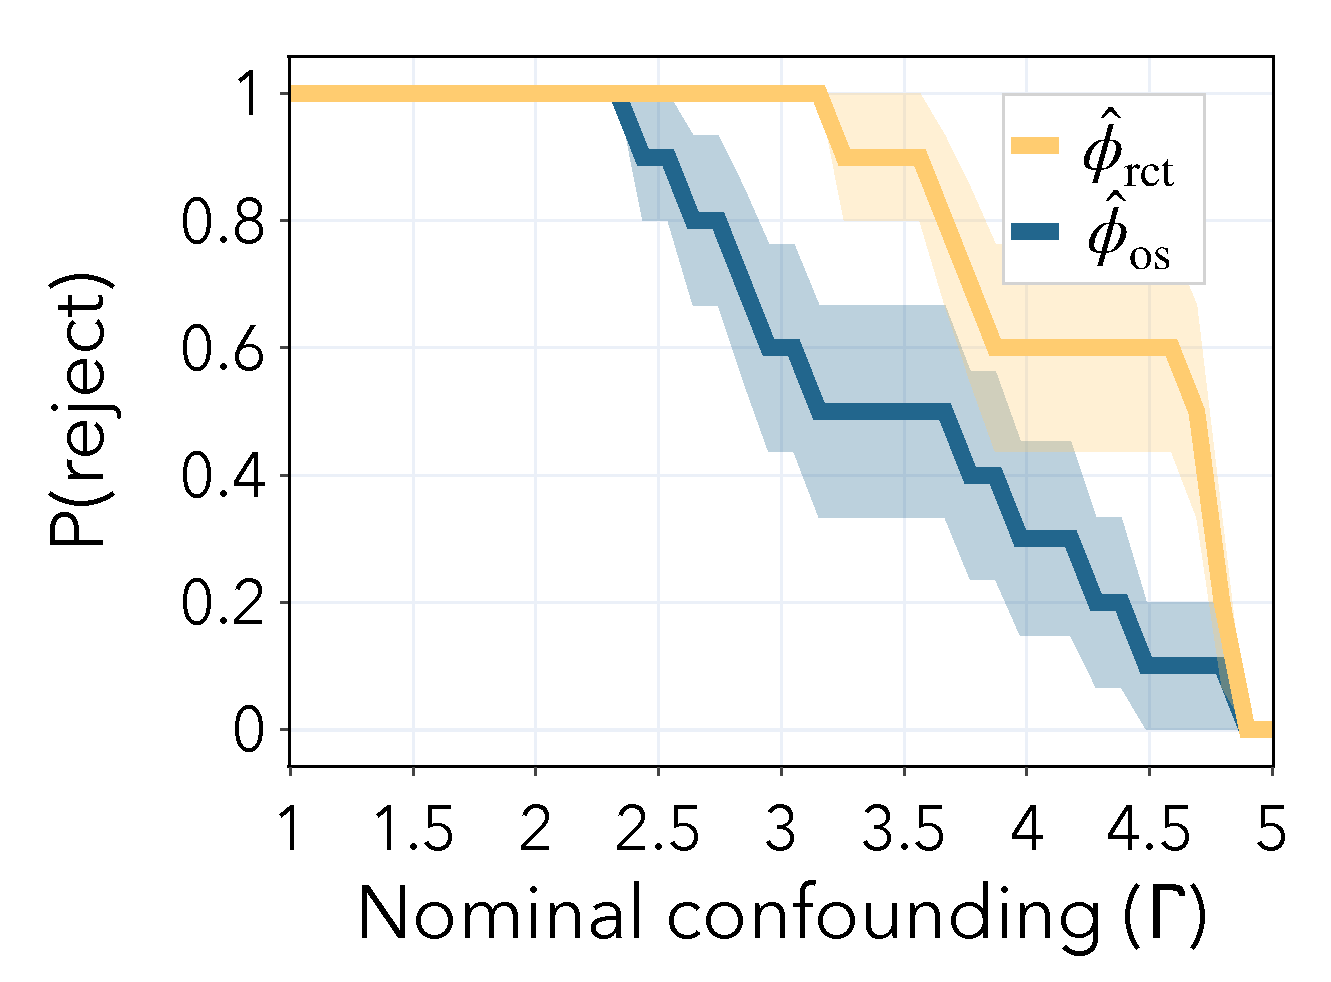
\includegraphics[width=\textwidth]{star_strong.pdf}
        \caption{Strong confounder: $Y$}
        \label{star:strong}

    \end{subfigure}
    
    \caption{Probability of rejection for different choices of $\confvalue$ for the test for the STAR Project. For all the plots, the significance level is $\alpha=0.05$ and $\Gammatrue=5$. We use the original sample sizes $\nrct=600,\nobs=1.8K$. (a) weak confounder: ``free lunch" (b) strong confounder: outcome $Y$.
 }
    \label{fig:star_results}
\end{figure*}